%% This is file `elsarticle-template-1-num.tex',
%%
%% Copyright 2009 Elsevier Ltd
%%
%% This file is part of the 'Elsarticle Bundle'.
%% ---------------------------------------------
%%
%% It may be distributed under the conditions of the LaTeX Project Public
%% License, either version 1.2 of this license or (at your option) any
%% later version.  The latest version of this license is in
%%    http://www.latex-project.org/lppl.txt
%% and version 1.2 or later is part of all distributions of LaTeX
%% version 1999/12/01 or later.
%%
%% Template article for Elsevier's document class `elsarticle'
%% with numbered style bibliographic references
%%
%% $Id: elsarticle-template-1-num.tex 149 2009-10-08 05:01:15Z rishi $
%% $URL: http://lenova.river-valley.com/svn/elsbst/trunk/elsarticle-template-1-num.tex $
%%
\documentclass[review,12pt]{elsarticle}

%% Use the option review to obtain double line spacing
%% \documentclass[preprint,review,12pt]{elsarticle}

%% Use the options 1p,twocolumn; 3p; 3p,twocolumn; 5p; or 5p,twocolumn
%% for a journal layout:
%% \documentclass[final,1p,times]{elsarticle}
%% \documentclass[final,1p,times,twocolumn]{elsarticle}
%% \documentclass[final,3p,times]{elsarticle}
%% \documentclass[final,3p,times,twocolumn]{elsarticle}
%% \documentclass[final,5p,times]{elsarticle}
%% \documentclass[final,5p,times,twocolumn]{elsarticle}

%% The graphicx package provides the includegraphics command.
\usepackage{graphicx}
%% The amssymb package provides various useful mathematical symbols
\usepackage{amssymb}
\usepackage{amsmath}
%% The amsthm package provides extended theorem environments
%% \usepackage{amsthm}

\usepackage{multirow}
\usepackage{url}

%% The lineno packages adds line numbers. Start line numbering with
%% \begin{linenumbers}, end it with \end{linenumbers}. Or switch it on
%% for the whole article with \linenumbers after \end{frontmatter}.
\usepackage{lineno}

%% natbib.sty is loaded by default. However, natbib options can be
%% provided with \biboptions{...} command. Following options are
%% valid:

%%   round  -  round parentheses are used (default)
%%   square -  square brackets are used   [option]
%%   curly  -  curly braces are used      {option}
%%   angle  -  angle brackets are used    <option>
%%   semicolon  -  multiple citations separated by semi-colon
%%   colon  - same as semicolon, an earlier confusion
%%   comma  -  separated by comma
%%   numbers-  selects numerical citations
%%   super  -  numerical citations as superscripts
%%   sort   -  sorts multiple citations according to order in ref. list
%%   sort&compress   -  like sort, but also compresses numerical citations
%%   compress - compresses without sorting
%%
%% \biboptions{comma,round}

% \biboptions{}

\graphicspath{{Figures/}}

\journal{ASHRAE Transactions}

\begin{document}

\begin{frontmatter}

%% Title, authors and addresses

\title{Characterization, Testing and Optimization of Load Aggregation Methods for Ground Heat Exchanger Response-Factor Models}

%% use the tnoteref command within \title for footnotes;
%% use the tnotetext command for the associated footnote;
%% use the fnref command within \author or \address for footnotes;
%% use the fntext command for the associated footnote;
%% use the corref command within \author for corresponding author footnotes;
%% use the cortext command for the associated footnote;
%% use the ead command for the email address,
%% and the form \ead[url] for the home page:
%%
%% \title{Title\tnoteref{label1}}
%% \tnotetext[label1]{}
%% \author{Name\corref{cor1}\fnref{label2}}
%% \ead{email address}
%% \ead[url]{home page}
%% \fntext[label2]{}
%% \cortext[cor1]{}
%% \address{Address\fnref{label3}}
%% \fntext[label3]{}


%% use optional labels to link authors explicitly to addresses:
%% \author[label1,label2]{<author name>}
%% \address[label1]{<address>}
%% \address[label2]{<address>}

\author[label1]{Matt Mitchell\corref{cor1}}
\author[label1]{Jeffrey Spitler}
\author[label2]{Edwin Lee}

\address[label1]{Oklahoma State University, Stillwater OK.}
\address[label2]{National Renewable Energy Laboratory, Golden CO.}

\cortext[cor1]{Corresponding author: matt.s.mitchell@okstate.edu}

\begin{abstract}
%% Text of abstract
This paper describes work performed to characterize and optimize the currently available load aggregation methods. A parametric study was performed by simulating several thousand test cases for different aggregation methods. The optimized methods and parameters for each respective algorithm are given.
\end{abstract}

\begin{keyword}
Ground heat exchanger, simulation, load aggregation, g-function
\end{keyword}

\end{frontmatter}

%%
%% Start line numbering here if you want
%%
\linenumbers

%% main text
\section*{Introduction}
Ground source heat pump (GSHP) systems are used to provide building space heating and cooling and hot water generation. The GSHP system heat pump is coupled to the soil via a ground heat exchanger (GHE), which is the heat sink/source for the system. This GSHP system exchanges energy between the heat pump and the soil via the GHE to provide for the heating and cooling loads. Below a certain depth (which varies with geography and location) the soil temperature remains constant during the year. This temperature is typically lower than the local ambient air temperature during periods of peak cooling demand, and higher than the ambient air temperature during periods of peek heating demand. As a result, GSHP systems can generally provide heating or cooling more efficiently than by using other more conventional heating and cooling technologies. 

GSHP systems \textit{can} be an effective and economical method for providing space heating and cooling. However, due to the complex nature of the thermally interacting ground heat exchangers, they are often difficult to apply rule-of-thumb based design approaches, as could more easily be done with other heating and cooling technologies. If the ground heat exchanger is not designed properly, it can cause the entire system to fail to meet the load. Additionally, since the GHE represents potentially the largest single-item cost of a GSHP system, it is important for it to be designed properly.

Therefore, in order for GSHP systems to be compared against other comparable heating and cooling systems, designers need the ability to simulate the systems and compare the results. Due to this, a great amount of effort has been put towards developing simulation models for GSHP and GHE. Designers, however, not only expect that the simulations be accurate, but they also expect them to be executed quickly.

One such GHE model that is often used for performing hourly GHE simulations is the model originally developed by \cite{EskilsonClaesson1988}. This model relies on precomputed response factors and the GHE load history to compute the temperature response of the GHE. Response factor type models are typically formulated as is shown in Equation \ref{eq:MFT}.

\begin{equation}
    T_f = T_g + \sum_{i=1}^n \frac{q_{i} - q_{i-1}}{2 \cdot \pi \cdot k_g} \cdot g\left(\frac{t_n - t_{i-1}}{t_s}\right) +  q_n \cdot R_b
    \label{eq:MFT}
\end{equation}

where:
\begin{flalign*}
    T_f &=\mbox{GHE mean-fluid temperature} && \\
    T_g &=\mbox{ground temperature} && \\
    q_i &=i^{th} \mbox{ GHE heat transfer rate normalized based on GHE length. i.e Btu/h-ft, W/m} && \\
    t_i &=i^{th} \mbox{ timestep} && \\
    t_s &=\mbox{ GHE time constant } \left(\frac{H^2}{9\cdot\alpha_g}\right) && \\
    R_b &=\mbox{ borehole thermal resistance} && \\
    g &=\mbox{g-function response factors} && \\
\end{flalign*}

At a fundamental level, conduction problems can be evaluated using linear partial differential equations. Because no non-linear terms exist in these equations, the principle of superpostion can be applied to simplify the solution. GHE response factor models take advantage of this property and apply the principle of superposition to compute the GHE temperature response by using the GHE load history. The GHE load history is treated as a series of step heat pulses which when superimposed and combined using the response factors can lead to an accurate calculation of the GHE temperature response. This reduces the solution of the fundamental conduction differential equations to the simple algebraic equation shown in Equation \ref{eq:MFT}.

A practical issue that arises from this superpostion approach, however, is the fact that the number of superposition calculations grows with the square of the number of timesteps \citep{YavuzturkSpitler1999}. Therefore, applying this approach directly will greatly affect simulation runtime. Attempting to simulate, say, for example an hourly annual or hourly multi-year simulations may be impractical without some way to reduce the number of computations required.

In order to reduce runtime, load aggregation procedures have been developed which will reduce then number of superposition calculations. This will in turn reduce simulation runtime. Load aggregation is the process of taking discrete individual loads that occurred over a given time interval, and replacing them with a single load over the same time interval. If the individual loads occurred over uniform timestep intervals, the average load rate could be computed and applied for the aggregated load. If the loads have non-uniform timesteps, and energy bases approach should be taken to ensure that energy is conserved.

As stated, several different load aggregation methods have been proposed, however, there has not been a direct comparison of all methods. Additionally, none of the existing methods have had their parameters optimized with the goal of minimizing simulation runtime and maximizing accuracy. This paper describe the process used to test these aggregation algorithms. It also recommends the best algorithm and the parameters for each algorithm which yield an acceptable balance of runtime saving and accuracy. The source code for this project is available here: \url{https://github.com/mitchute/GLHE}

\section*{Methods}

\subsection*{Static Method}

Several different load aggregation procedures have been proposed. These will be outlined and described here. The methods used to compare the methods will also be described.

\cite{YavuzturkSpitler1999} were the first to develop a load aggregation procedure to reduce simulation runtime. The method relies on using ``monthly" heat pulses to aggregate 730 hourly loads, though the method retains 192 hourly heat pulses for the most recent 192 simulation hours. In other words, once the first 922 (192 + 730) hours have passed, the 730 hours which are farthest from the current simulation time are aggregated into monthly blocks. Once another 730 hours have passed the next 730 hours are aggregated into another monthly block. This process is repeated for the duration of the simulation.

To further illustrate this example, once 922 (192 + 730) simulated hours have passed, the hourly loads from hour 730 to 0 are aggregated together into a single block. The mean value of the loads over this period is computed and the 730 individual hourly loads are removed and replaced with a single value. This single value represents the average load over this 730 hour period. As the simulation continues for another 730 hours until hour 1652, the hourly loads from hours 1461 to 731 are aggregated together again into another monthly block.

The test parameter for this method are given in Table \ref{tab:static cases}. Case a shows the duration of the bin in hours, and case 1 shows the minimum number of bins which were were held. In this case, we have 192 hourly loads which are held, which are then aggregated into 730 hour bins when possible.

\begin{table}[htbp!]
\centering
\caption{Static method simulation case descriptions}
\label{tab:static cases}
\begin{tabular}{ccc}
Case                    & \multicolumn{2}{c}{Bin Duration (hr)}               \\ \hline
\multicolumn{1}{|c|}{a} & \multicolumn{1}{c|}{1}   & \multicolumn{1}{c|}{730} \\ \hline
                        &                          &                          \\
Case                    & \multicolumn{2}{c}{Min Num. Bins}                   \\ \hline
\multicolumn{1}{|c|}{1} & \multicolumn{1}{c|}{192} & \multicolumn{1}{c|}{1}   \\ \hline
\end{tabular}
\end{table}
The authors state that they tested the minimum hourly history periods of 24, 192, and 730 hours. However, the method is not stated to have been optimized any further. As a result, a question that arises is that of whether the minimum of 192 hourly loads and 730 hour ``monthly" blocks will result in the best performance?

Fundamentally, this method forms the basis for what is termed the ``static" method. The method is characterized by smaller load blocks which collapse into larger blocks once a sufficient number of the smaller blocks have been created. This was illustrated in the above example when the smaller hourly load blocks collapsed into the larger 730 hour blocks after a sufficient number of smaller blocks have been created. 

The method could loosely be thought of as similar to the Lagrangian approach which, in the case of fluid flow characterizations, tracks individual particles or packets of fluid, rather than tracking a fixed control volume through which fluid flows. In our case, however, we are concerned with tracking individual loads or load blocks which are formed from previously aggregated smaller blocks. These load blocks are created and added to our resistance factor calculations. Once a sufficient number of the blocks have been created, they collapse into a larger block. After a load block is formed, the load values remain within the block until the block is aggregated together with other similar blocks.

To illustrate this, consider the example given in Table \ref{tab:static example}. In this example, we will assume that the timesteps have a value of $h$, and that we will keep a minimum of three $h$ before aggregating into $2h$ blocks.

\begin{table}[htbp!]
\centering
\caption{Static method aggregation example.}
\label{tab:static example}
\begin{tabular}{cccccc}
Bin No.                                  & 1                      & 2                      & 3                      & 4                        & 5                        \\
Timestep                                 &                        &                        &                        &                          &                          \\ \cline{1-2}
\multicolumn{1}{|c|}{\multirow{2}{*}{1}} & \multicolumn{1}{c|}{h} &                        &                        &                          &                          \\ \cline{2-2}
\multicolumn{1}{|c|}{}                   & \multicolumn{1}{c|}{1} &                        &                        &                          &                          \\ \cline{1-2}
                                         &                        &                        &                        &                          &                          \\ \cline{1-3}
\multicolumn{1}{|c|}{\multirow{2}{*}{2}} & \multicolumn{1}{c|}{h} & \multicolumn{1}{c|}{h} &                        &                          &                          \\ \cline{2-3}
\multicolumn{1}{|c|}{}                   & \multicolumn{1}{c|}{0} & \multicolumn{1}{c|}{1} &                        &                          &                          \\ \cline{1-3}
                                         &                        &                        &                        &                          &                          \\ \cline{1-4}
\multicolumn{1}{|c|}{\multirow{2}{*}{3}} & \multicolumn{1}{c|}{h} & \multicolumn{1}{c|}{h} & \multicolumn{1}{c|}{h} &                          &                          \\ \cline{2-4}
\multicolumn{1}{|c|}{}                   & \multicolumn{1}{c|}{0} & \multicolumn{1}{c|}{0} & \multicolumn{1}{c|}{1} &                          &                          \\ \cline{1-4}
                                         &                        &                        &                        &                          &                          \\ \cline{1-5}
\multicolumn{1}{|c|}{\multirow{2}{*}{4}} & \multicolumn{1}{c|}{h} & \multicolumn{1}{c|}{h} & \multicolumn{1}{c|}{h} & \multicolumn{1}{c|}{h}   &                          \\ \cline{2-5}
\multicolumn{1}{|c|}{}                   & \multicolumn{1}{c|}{0} & \multicolumn{1}{c|}{0} & \multicolumn{1}{c|}{0} & \multicolumn{1}{c|}{1}   &                          \\ \cline{1-5}
                                         &                        &                        &                        &                          &                          \\ \cline{1-5}
\multicolumn{1}{|c|}{\multirow{2}{*}{5}} & \multicolumn{1}{c|}{h} & \multicolumn{1}{c|}{h} & \multicolumn{1}{c|}{h} & \multicolumn{1}{c|}{2h}  &                          \\ \cline{2-5}
\multicolumn{1}{|c|}{}                   & \multicolumn{1}{c|}{0} & \multicolumn{1}{c|}{0} & \multicolumn{1}{c|}{0} & \multicolumn{1}{c|}{1/2} &                          \\ \cline{1-5}
                                         &                        &                        &                        &                          &                          \\ \hline
\multicolumn{1}{|c|}{\multirow{2}{*}{6}} & \multicolumn{1}{c|}{h} & \multicolumn{1}{c|}{h} & \multicolumn{1}{c|}{h} & \multicolumn{1}{c|}{h}   & \multicolumn{1}{c|}{2h}  \\ \cline{2-6} 
\multicolumn{1}{|c|}{}                   & \multicolumn{1}{c|}{0} & \multicolumn{1}{c|}{0} & \multicolumn{1}{c|}{0} & \multicolumn{1}{c|}{0}   & \multicolumn{1}{c|}{1/2} \\ \hline
                                         &                        &                        &                        &                          &                          \\ \hline
\multicolumn{1}{|c|}{\multirow{2}{*}{7}} & \multicolumn{1}{c|}{h} & \multicolumn{1}{c|}{h} & \multicolumn{1}{c|}{h} & \multicolumn{1}{c|}{2h}  & \multicolumn{1}{c|}{2h}  \\ \cline{2-6} 
\multicolumn{1}{|c|}{}                   & \multicolumn{1}{c|}{0} & \multicolumn{1}{c|}{0} & \multicolumn{1}{c|}{0} & \multicolumn{1}{c|}{0}   & \multicolumn{1}{c|}{1/2} \\ \hline
\end{tabular}
\end{table}

The steps occurring at each timestep are described below.

\begin{itemize}
    \item Timestep 1: a new load with a value of 1 occurs. This is placed in Bin 1.
    
    \item Timestep 2-4: the load from Bin 1 from the previous timestep is displaced to Bin 2. No new loads occurs at timestep 2, so a value of 0 is placed in Bin 1. This process is repeated for for the next two timesteps until Bins 1-3 each contain a value of 0, and Bin 4 has a value 1.
    
    \item Timestep 5: no new load occurs at timestep 5, so a value of 0 is place in Bin 1 and the other bins are displaced, so that Bins 1-4 contain a value of 0, and Bin 5 contains a value of 1. As was stated when the example was defined above, we plan to keep three $h$ loads and then aggregate into $2h$ blocks for any remaining loads. As a result, the loads from Bins 4-5 collapse into a $2h$ load block with a value of 1/2, since this is the average load over this time period.
    
    \item Timestep 6: no new load occurs, so a value of 0 is placed in Bin 1 and the other bins are displaced.
    
    \item Timestep 7: no new load occurs, so a value of 0 is placed in Bin 1 and the other bins are displaced. Bins 4-5 are again aggregated into a single bin of width $2h$.
    
\end{itemize}

\cite{Liu2005} developed another static load aggregation scheme, which is stated to be an improvement on the method by \cite{YavuzturkSpitler1999}. The author referred to the scheme as a ``hierarchical" approach, which used the following parameters to guide the aggregation process.

\begin{itemize}
    \item A minimum of 12 hourly loads are kept for the 12 most recently simulated hours.

    \item Hourly loads are then aggregated into daily, 24 hour blocks. These blocks are referred to as ``small" blocks.

    \item Five ``small" blocks are aggregated into ``medium" blocks with a minimum of three small blocks kept after the aggregation process. In other words, once eight small blocks have been created, the five which are most distant from the current simulation time are aggregated into medium blocks to represent a period of 120 hours.
    
    \item 73 ``medium" blocks are then aggregated into ``large" blocks which represents 8760 simulation hours, with 40 medium blocks to be kept unaggregated. In other words, once 113 medium blocks have been created, the 73 which are most distant from the current simulation time are aggregated into a period of 8760 hours.
    
\end{itemize}

These are summarized in the simulation case descriptions in Table \ref{tab: hierarchical cases}.

\begin{table}[htbp!]
\centering
\caption{Hierarchical method simulation case descriptions}
\label{tab: hierarchical cases}
\begin{tabular}{ccccc}
Case                    & \multicolumn{4}{c}{Bin Duration (hr)}                                                                    \\ \hline
\multicolumn{1}{|c|}{a} & \multicolumn{1}{c|}{1}  & \multicolumn{1}{c|}{24} & \multicolumn{1}{c|}{120} & \multicolumn{1}{c|}{8760} \\ \hline
                        &                         &                         &                          &                           \\
Case                    & \multicolumn{4}{c}{Min Num. Bins}                                                                        \\ \hline
\multicolumn{1}{|c|}{1} & \multicolumn{1}{c|}{12} & \multicolumn{1}{c|}{3}  & \multicolumn{1}{c|}{40}  & \multicolumn{1}{c|}{1}    \\ \hline
\end{tabular}
\end{table}

The author claims that the method results in generating only 12\% of the aggregation block when compared to the \cite{YavuzturkSpitler1999} method, and that this results in a 20\% reduction in simulation time.

\cite{BernierPinelLabibPaillot2004} also developed another static aggregation algorithm which was termed the ``multiple-load aggregation algorithm" (MLAA). The method uses a GHE model formulation which relies on a cylindrical heat source equation, rather than the response factor approach outlined previously. Regardless, of this, the load aggregation procedure which is described is applicable to the work performed here.

The authors tested a number of different variations for bin duration, but settled on the following:

\begin{itemize}
    \item A minimum of 12 hourly values are kept.
    
    \item Hourly values are aggregated into blocks representing 48 hours, termed ``daily" blocks.

    \item Daily blocks are aggregated into 168 hour ``weekly" blocks.
    
    \item Weekly blocks are aggregated into 360 hour ``monthly" blocks.

\end{itemize}

Something that should be pointed out regarding this work's testing of the MLAA method, is the fact that the aggregation blocks specified by the authors do not aggregate together evenly. As the method is formulated in this work, the aggregation blocks must be integer combinations of each other. In other words, we can take, for example, 3 or 4 smaller blocks and combine them together to form a larger block, but we cannot take 3.2 smaller blocks to form a larger block. In the case of the MLAA algorithm, the 48 is not an integer multiple of 168, so this discrepancy causes a minor implementation issue. 

The authors also do not say whether any holding periods were used besides the one mentioned for the hourly loads. Therefore, for this work small range of holding periods were tested.

To get around the problem, simulation cases were created to bracket the intervals specified by the authors. These are specified below in Table \ref{tab:MLAA cases}. Cases a-c show the duration of each bin in hours, and cases 1-4 show the minimum number of bins which will be held unaggregated. All combinations of cases a-c and 1-4 were run in an attempt to bracket the original method.

\begin{table}[htbp!]
\centering
\caption{MLAA simulation case descriptions}
\label{tab:MLAA cases}
\begin{tabular}{ccccc}
Case                    & \multicolumn{4}{c}{Bin Duration (hr)}                                                                   \\ \hline
\multicolumn{1}{|c|}{a} & \multicolumn{1}{c|}{1}  & \multicolumn{1}{c|}{48} & \multicolumn{1}{c|}{144} & \multicolumn{1}{c|}{432} \\ \hline
\multicolumn{1}{|c|}{b} & \multicolumn{1}{c|}{1}  & \multicolumn{1}{c|}{48} & \multicolumn{1}{c|}{144} & \multicolumn{1}{c|}{288} \\ \hline
\multicolumn{1}{|c|}{c} & \multicolumn{1}{c|}{1}  & \multicolumn{1}{c|}{48} & \multicolumn{1}{c|}{192} & \multicolumn{1}{c|}{384} \\ \hline
                        &                         &                         &                          &                          \\
Case                    & \multicolumn{4}{c}{Min Num. Bins}                                                                             \\ \hline
\multicolumn{1}{|c|}{1} & \multicolumn{1}{c|}{12} & \multicolumn{1}{c|}{4}  & \multicolumn{1}{c|}{3}   & \multicolumn{1}{c|}{3}   \\ \hline
\multicolumn{1}{|c|}{2} & \multicolumn{1}{c|}{12} & \multicolumn{1}{c|}{4}  & \multicolumn{1}{c|}{3}   & \multicolumn{1}{c|}{2}   \\ \hline
\multicolumn{1}{|c|}{3} & \multicolumn{1}{c|}{12} & \multicolumn{1}{c|}{4}  & \multicolumn{1}{c|}{4}   & \multicolumn{1}{c|}{3}   \\ \hline
\multicolumn{1}{|c|}{4} & \multicolumn{1}{c|}{12} & \multicolumn{1}{c|}{1}  & \multicolumn{1}{c|}{1}   & \multicolumn{1}{c|}{1}   \\ \hline
\end{tabular}
\end{table}

One observable disadvantage of the static method is that it is difficult to store and reuse g-function response factors once they have been computed. As is seen in Equation \ref{eq:MFT}, the g-function is referenced from the current simulation time to the end of the bin for which you are computing within the summation term. Pre-computing and reusing g-functions for the first set of bins is not a problem, but issue arise for subsequent bins. Because duration of bins can be any integer multiple of the previous bin's duration, and each bin level can have any arbitrary number of holding periods, it becomes extremely difficult to determine beforehand the time intervals for which g-functions will be needed. Therefore, it is easier to simply compute the g-functions as needed at the beginning of each timestep rather than attempting to precompute and store them.

An example of this can be seen by referring back to Table \ref{tab:static example}. Response factors for Bins 1-3 could easily be stored and reused. However, for subsequent bins, the end time of each bin varies at each timestep. For example, at timestep 4 Bin 4 ends at at the end of $4h$ timesteps. Advancing to timestep 5, Bin 4 now ends at timestep $5h$, thus requiring the g-function be recomputed. Advancing again at timestep 6, the Bin 4 now ends again back at $4h$. This effect cascades up through the list of bins and with additional bin duration and holding periods become extreemly difficult to track. It is simply easier to recompute the g-function rather than determining which of all possible combinations of g-functions to store and retrieve.

Besides the previously described methods \citep{YavuzturkSpitler1999, BernierPinelLabibPaillot2004, Liu2005} a parametric study was performed by varying the parameters of the static method over a wide range. These parameters are shows in Table \ref{tab:static case durations} and Table \ref{tab:staic case nums}. 

In Table \ref{tab:static case durations}, we can see that cases a-v show the duration of each bin level. Starting with case a, the bins increase at with a $2\times$ multiplier, starting from an hourly level of 1 hour, then increasing to 2, 4, 8, etc. Case b uses a $3\times$ multiplier; case c uses a $4\times$ multiplier; etc.

In Table \ref{tab:staic case nums}, we can see the minimum number of hourly bins, and the minimum number of the remaining bins which will need to be held before any aggregation can occur. Cases 1-12 show the minimum number of hourly bins, and cases $\alpha$, $\beta$, $\gamma$, and $\delta$ indicate the minimum number of the remaining bins.

In total, 1056 case combinations represent the static method parametric study.

\begin{table}[htbp!]
\centering
\caption{Static method parametric study simulation case durations}
\label{tab:static case durations}
\begin{tabular}{cccccccccccc}
Case                                     & \multicolumn{11}{c}{Bin Duration (hr)}                                                                                                                                                                                                                                                                             \\ \hline
\multicolumn{1}{|c|}{\multirow{2}{*}{a}} & \multicolumn{1}{c|}{1} & \multicolumn{1}{c|}{2}  & \multicolumn{1}{c|}{4}   & \multicolumn{1}{c|}{8}     & \multicolumn{1}{c|}{16}    & \multicolumn{1}{c|}{32}    & \multicolumn{1}{c|}{64}    & \multicolumn{1}{c|}{128}   & \multicolumn{1}{c|}{256}  & \multicolumn{1}{c|}{512}   & \multicolumn{1}{c|}{1024}  \\ \cline{2-12} 
\multicolumn{1}{|c|}{}                   &                        &                         &                          &                            &                            &                            & \multicolumn{1}{c|}{}      & \multicolumn{1}{c|}{2048}  & \multicolumn{1}{c|}{4096} & \multicolumn{1}{c|}{8192}  & \multicolumn{1}{c|}{16384} \\ \hline
\multicolumn{1}{|c|}{b}                  & \multicolumn{1}{c|}{1} & \multicolumn{1}{c|}{3}  & \multicolumn{1}{c|}{9}   & \multicolumn{1}{c|}{27}    & \multicolumn{1}{c|}{81}    & \multicolumn{1}{c|}{243}   & \multicolumn{1}{c|}{729}   & \multicolumn{1}{c|}{2187}  & \multicolumn{1}{c|}{6561} & \multicolumn{1}{c|}{19683} &                            \\ \cline{1-11}
\multicolumn{1}{|c|}{c}                  & \multicolumn{1}{c|}{1} & \multicolumn{1}{c|}{4}  & \multicolumn{1}{c|}{16}  & \multicolumn{1}{c|}{64}    & \multicolumn{1}{c|}{256}   & \multicolumn{1}{c|}{1024}  & \multicolumn{1}{c|}{4096}  & \multicolumn{1}{c|}{16384} &                           &                            &                            \\ \cline{1-9}
\multicolumn{1}{|c|}{d}                  & \multicolumn{1}{c|}{1} & \multicolumn{1}{c|}{5}  & \multicolumn{1}{c|}{25}  & \multicolumn{1}{c|}{125}   & \multicolumn{1}{c|}{625}   & \multicolumn{1}{c|}{3125}  & \multicolumn{1}{c|}{15625} &                            &                           &                            &                            \\ \cline{1-8}
\multicolumn{1}{|c|}{e}                  & \multicolumn{1}{c|}{1} & \multicolumn{1}{c|}{7}  & \multicolumn{1}{c|}{49}  & \multicolumn{1}{c|}{343}   & \multicolumn{1}{c|}{2401}  & \multicolumn{1}{c|}{16807} &                            &                            &                           &                            &                            \\ \cline{1-7}
\multicolumn{1}{|c|}{f}                  & \multicolumn{1}{c|}{1} & \multicolumn{1}{c|}{8}  & \multicolumn{1}{c|}{64}  & \multicolumn{1}{c|}{512}   & \multicolumn{1}{c|}{4096}  &                            &                            &                            &                           &                            &                            \\ \cline{1-6}
\multicolumn{1}{|c|}{g}                  & \multicolumn{1}{c|}{1} & \multicolumn{1}{c|}{9}  & \multicolumn{1}{c|}{81}  & \multicolumn{1}{c|}{729}   & \multicolumn{1}{c|}{6561}  &                            &                            &                            &                           &                            &                            \\ \cline{1-6}
\multicolumn{1}{|c|}{h}                  & \multicolumn{1}{c|}{1} & \multicolumn{1}{c|}{10} & \multicolumn{1}{c|}{100} & \multicolumn{1}{c|}{1000}  & \multicolumn{1}{c|}{10000} &                            &                            &                            &                           &                            &                            \\ \cline{1-6}
\multicolumn{1}{|c|}{i}                  & \multicolumn{1}{c|}{1} & \multicolumn{1}{c|}{11} & \multicolumn{1}{c|}{121} & \multicolumn{1}{c|}{1331}  & \multicolumn{1}{c|}{14641} &                            &                            &                            &                           &                            &                            \\ \cline{1-6}
\multicolumn{1}{|c|}{j}                  & \multicolumn{1}{c|}{1} & \multicolumn{1}{c|}{12} & \multicolumn{1}{c|}{144} & \multicolumn{1}{c|}{1728}  & \multicolumn{1}{c|}{20736} &                            &                            &                            &                           &                            &                            \\ \cline{1-6}
\multicolumn{1}{|c|}{k}                  & \multicolumn{1}{c|}{1} & \multicolumn{1}{c|}{13} & \multicolumn{1}{c|}{169} & \multicolumn{1}{c|}{2197}  &                            &                            &                            &                            &                           &                            &                            \\ \cline{1-5}
\multicolumn{1}{|c|}{l}                  & \multicolumn{1}{c|}{1} & \multicolumn{1}{c|}{14} & \multicolumn{1}{c|}{196} & \multicolumn{1}{c|}{2744}  &                            &                            &                            &                            &                           &                            &                            \\ \cline{1-5}
\multicolumn{1}{|c|}{m}                  & \multicolumn{1}{c|}{1} & \multicolumn{1}{c|}{15} & \multicolumn{1}{c|}{225} & \multicolumn{1}{c|}{3375}  &                            &                            &                            &                            &                           &                            &                            \\ \cline{1-5}
\multicolumn{1}{|c|}{n}                  & \multicolumn{1}{c|}{1} & \multicolumn{1}{c|}{16} & \multicolumn{1}{c|}{256} & \multicolumn{1}{c|}{4096}  &                            &                            &                            &                            &                           &                            &                            \\ \cline{1-5}
\multicolumn{1}{|c|}{o}                  & \multicolumn{1}{c|}{1} & \multicolumn{1}{c|}{17} & \multicolumn{1}{c|}{289} & \multicolumn{1}{c|}{4913}  &                            &                            &                            &                            &                           &                            &                            \\ \cline{1-5}
\multicolumn{1}{|c|}{p}                  & \multicolumn{1}{c|}{1} & \multicolumn{1}{c|}{18} & \multicolumn{1}{c|}{324} & \multicolumn{1}{c|}{5832}  &                            &                            &                            &                            &                           &                            &                            \\ \cline{1-5}
\multicolumn{1}{|c|}{q}                  & \multicolumn{1}{c|}{1} & \multicolumn{1}{c|}{19} & \multicolumn{1}{c|}{361} & \multicolumn{1}{c|}{6859}  &                            &                            &                            &                            &                           &                            &                            \\ \cline{1-5}
\multicolumn{1}{|c|}{r}                  & \multicolumn{1}{c|}{1} & \multicolumn{1}{c|}{20} & \multicolumn{1}{c|}{400} & \multicolumn{1}{c|}{8000}  &                            &                            &                            &                            &                           &                            &                            \\ \cline{1-5}
\multicolumn{1}{|c|}{s}                  & \multicolumn{1}{c|}{1} & \multicolumn{1}{c|}{21} & \multicolumn{1}{c|}{441} & \multicolumn{1}{c|}{9261}  &                            &                            &                            &                            &                           &                            &                            \\ \cline{1-5}
\multicolumn{1}{|c|}{t}                  & \multicolumn{1}{c|}{1} & \multicolumn{1}{c|}{22} & \multicolumn{1}{c|}{484} & \multicolumn{1}{c|}{10648} &                            &                            &                            &                            &                           &                            &                            \\ \cline{1-5}
\multicolumn{1}{|c|}{u}                  & \multicolumn{1}{c|}{1} & \multicolumn{1}{c|}{23} & \multicolumn{1}{c|}{529} & \multicolumn{1}{c|}{12167} &                            &                            &                            &                            &                           &                            &                            \\ \cline{1-5}
\multicolumn{1}{|c|}{v}                  & \multicolumn{1}{c|}{1} & \multicolumn{1}{c|}{24} & \multicolumn{1}{c|}{576} & \multicolumn{1}{c|}{13824} &                            &                            &                            &                            &                           &                            &                            \\ \cline{1-5}
\end{tabular}
\end{table}

\begin{table}[htbp!]
\centering
\caption{Static method parametric study minimum number of bins}
\label{tab:staic case nums}
\begin{tabular}{|c|c|ccc}
\cline{1-2} \cline{4-5}
Case & Min.~Num.~Hourly Bins & \multicolumn{1}{c|}{} & \multicolumn{1}{c|}{Case}                  & \multicolumn{1}{c|}{Min.~Num.~Other Bins} \\ \cline{1-2} \cline{4-5} 
1    & 4                     & \multicolumn{1}{c|}{} & \multicolumn{1}{c|}{$\alpha$} & \multicolumn{1}{c|}{4}                    \\ \cline{1-2} \cline{4-5} 
2    & 8                     & \multicolumn{1}{c|}{} & \multicolumn{1}{c|}{$\beta$}  & \multicolumn{1}{c|}{6}                    \\ \cline{1-2} \cline{4-5} 
3    & 10                    & \multicolumn{1}{c|}{} & \multicolumn{1}{c|}{$\gamma$} & \multicolumn{1}{c|}{8}                    \\ \cline{1-2} \cline{4-5} 
4    & 20                    & \multicolumn{1}{c|}{} & \multicolumn{1}{c|}{$\delta$} & \multicolumn{1}{c|}{10}                   \\ \cline{1-2} \cline{4-5} 
5    & 30                    &                       &                                            &                                           \\ \cline{1-2}
6    & 40                    &                       &                                            &                                           \\ \cline{1-2}
7    & 50                    &                       &                                            &                                           \\ \cline{1-2}
8    & 60                    &                       &                                            &                                           \\ \cline{1-2}
9    & 70                    &                       &                                            &                                           \\ \cline{1-2}
10   & 80                    &                       &                                            &                                           \\ \cline{1-2}
11   & 90                    &                       &                                            &                                           \\ \cline{1-2}
12   & 100                   &                       &                                            &                                           \\ \cline{1-2}
\end{tabular}
\end{table}

\subsection*{Dynamic Method}

\cite{ClaessonJaved2012} is the most recent load aggregation method to have been developed. The method, as opposed to the ``static" method described previously, follows what could be characterized as an Eulerian approach. In a fluid flow application, the flow through a fixed control volume is assessed rather than individual packets or particles of fluid. In our case, we predefine the bins and allow energy (GHE loads) to move through the bins.  This is illustrated in Table \ref{tab:dynamic example}, which is an example taken from \cite{ClaessonJaved2012}. 

In the table the values of the GHE loads for each timestep within each bin is represented. Horizontally, the bin widths are are given as h or 2h, where h represent the length of the timestep. The most recent load is always in the first bin. See the following description:

\begin{itemize}
    \item At timestep 1, a value of 1 is placed in the Bin 1. 
    
    \item At timestep 2, $h \times 1/h \times$ 1 is moved from Bin 1 to Bin 2. In other words, the timestep length, times the inverse of the current bin width, times the value of the energy in bin itself is moved from Bin 1 to Bin 2. In this case, the timestep is h, the bin width is h, and the value of the energy in Bin 1 is 1, so 100\% of the energy (1) is moved from Bin 1 to Bin 2.  Energy is conserved and since the bins have the same width (meaning they represent the same time interval), the new value of Bin 2 is 1.
    
    \item At timestep 3, the same process is repeated. $h \times 1/h \times$ 1 is the value of energy which is moved from Bin 2 to Bin 3. However, Bin 3 has a width of $2h$, so the magnitude of the energy represented by the Bin is now 1/2. Again, energy is conserved but the original pulse of 1 is now assumed to have occurred over a $2h$ time interval. This process is repeated for all remaining timesteps.

\end{itemize}

\begin{table}[htbp!]
\centering
\caption{Dynamic aggregation example}
\label{tab:dynamic example}
\begin{tabular}{cccccccc}
Bin No.                 & 1                      & 2                      & 3                         & 4                         & 5                         & 6                         & 7                         \\
Width                   & h                      & h                      & 2h                        & 2h                        & 2h                        & 2h                        & 2h                        \\
Timestep                &                        &                        &                           &                           &                           &                           &                           \\ \cline{1-2}
\multicolumn{1}{|c|}{1} & \multicolumn{1}{c|}{1} &                        &                           &                           &                           &                           &                           \\ \cline{1-3}
\multicolumn{1}{|c|}{2} & \multicolumn{1}{c|}{0} & \multicolumn{1}{c|}{1} &                           &                           &                           &                           &                           \\ \cline{1-4}
\multicolumn{1}{|c|}{3} & \multicolumn{1}{c|}{0} & \multicolumn{1}{c|}{0} & \multicolumn{1}{c|}{1/2}  &                           &                           &                           &                           \\ \cline{1-5}
\multicolumn{1}{|c|}{4} & \multicolumn{1}{c|}{0} & \multicolumn{1}{c|}{0} & \multicolumn{1}{c|}{1/4}  & \multicolumn{1}{c|}{1/4}  &                           &                           &                           \\ \cline{1-6}
\multicolumn{1}{|c|}{5} & \multicolumn{1}{c|}{0} & \multicolumn{1}{c|}{0} & \multicolumn{1}{c|}{1/8}  & \multicolumn{1}{c|}{2/8}  & \multicolumn{1}{c|}{1/8}  &                           &                           \\ \cline{1-7}
\multicolumn{1}{|c|}{6} & \multicolumn{1}{c|}{0} & \multicolumn{1}{c|}{0} & \multicolumn{1}{c|}{1/16} & \multicolumn{1}{c|}{3/16} & \multicolumn{1}{c|}{3/16} & \multicolumn{1}{c|}{1/16} &                           \\ \hline
\multicolumn{1}{|c|}{7} & \multicolumn{1}{c|}{0} & \multicolumn{1}{c|}{0} & \multicolumn{1}{c|}{1/32} & \multicolumn{1}{c|}{4/32} & \multicolumn{1}{c|}{6/32} & \multicolumn{1}{c|}{4/32} & \multicolumn{1}{c|}{1/32} \\ \hline
\end{tabular}
\end{table}

Due to the fact that the bin widths are predetermined and are fixed relative to the current simulation time (i.e. in our above example bin 3, for example, will always represents the loads which occurred from 2-4 hours prior to the current simulation time), the g-function response factors can be precomputed. This eliminates the need to continuously compute these values at each timestep, as was the case with the static method.

However, another issue which arises due to this method is the fact that the load values diffuse with time. Not only do they diffuse with time (meaning the amplitude of the original value decreases with time), the load values also disperse into the GHE history faster than actually occurs. To illustrate this, let us consider the previous dynamic method example.

At timestep 7, the original load value of 1 is now smeared across 5 different bins. This example is similar to the example given for the static method, and in reality the value should be 1/2 and located within Bin 5. This illustrates the diffusive nature of the method. We can also see that the load value has propagated as far at $12h$ into the load history, since we have non-zero values in Bins 6-7. This illustrates the dispersive nature of the method.

In reality, we expect the hours which are most near to the current simulation time to have the largest effect on the GHE temperature response. We do not expect hourly load variations from, say, several days before the current simulation time to have a significant effect on the temperature response calculations. What is important, however, is that energy is conserved. As illustrated above, this method does conserve energy, so the results of the diffusion and dispersion errors may not cause significant simulation errors.

The for this implementation, the dynamic method can be characterized using two parameters; the expansion rate of the bin levels, and the number of bins at each level. The number of levels can be expanded as needed for fit the requirements of the duration of the simulation.

For reference, the implementation described by \cite{ClaessonJaved2012} uses an expansion rate of 2, and the number of bins as each level of 5. The authors also use 16 levels as this is more than sufficient to perform a 20 year simulation. This is illustrated in Table \ref{tab:claesson example}.

The duration of the bins within each level is indicated in the level bin duration column in Table \ref{tab:claesson example}. Here, the authors determine the duration of bins within each level with the following formula:

\begin{equation}
    r_q = c^{q - 1}
\end{equation}

where:
\begin{flalign*}
    r_q &=\mbox{ duration of each bin, in hours} && \\
    c &=\mbox{ expansion rate} && \\
    q &=\mbox{ level number} && \\
\end{flalign*}

\begin{table}[htbp!]
\centering
\caption{Dynamic method as proposed by \cite{ClaessonJaved2012}}
\label{tab:claesson example}
\begin{tabular}{|c|c|c|c|c|c|c|}
\hline
Level & Level Bin Duration & \multicolumn{5}{c|}{Simulation Hours}      \\ \hline
1     & h                  & 1      & 2      & 3      & 4      & 5      \\ \hline
2     & 2h                 & 7      & 9      & 11     & 13     & 15     \\ \hline
3     & 4h                 & 19     & 23     & 27     & 31     & 35     \\ \hline
4     & 8h                 & 43     & 51     & 59     & 67     & 75     \\ \hline
5     & 16h                & 91     & 107    & 123    & 139    & 155    \\ \hline
6     & 32h                & 187    & 219    & 251    & 283    & 315    \\ \hline
7     & 64h                & 379    & 443    & 507    & 571    & 635    \\ \hline
8     & 128h               & 763    & 891    & 1019   & 1147   & 1275   \\ \hline
9     & 256h               & 1531   & 1787   & 2043   & 2299   & 2555   \\ \hline
10    & 512h               & 3067   & 3579   & 4091   & 4603   & 5115   \\ \hline
11    & 1024h              & 6139   & 7163   & 8187   & 9211   & 10235  \\ \hline
12    & 2048h              & 12283  & 14331  & 16379  & 18427  & 20475  \\ \hline
13    & 4096h              & 24571  & 28667  & 32763  & 36859  & 40955  \\ \hline
14    & 8192h              & 49147  & 57339  & 65531  & 73723  & 81915  \\ \hline
15    & 16384h             & 98299  & 114683 & 131067 & 147451 & 163835 \\ \hline
16    & 32768h             & 196603 & 229371 & 262139 & 294907 & 327675 \\ \hline
\end{tabular}
\end{table}

The simulation hours columns indicates the end hour, in to the GHE load history for which that bin is applicable. Starting at level 1, the first bin (which has a value of 1) will account for the current simulation load. Moving right, next bin will account for the load from 1-2 hours into the GHE load history. This process is repeated until the end of the level.

At level 2, the first bin (which has a value of 7) accounts for loads from 5-7 hours into the GHE load history. The next bin accounts from hours 7-9, etc.

For the parametric study performed during this work the, expansion rate was varied from 1.25 to 3.0 at an interval of 0.25. However, the a value of $\frac{1+\sqrt{5}}{2} = 1.618\ldots$ (golden ratio) was also tested, for a total of 9 expansion rates. Starting and ending number of bin from 1-10 were also tested. In the example above, all levels have the number of bins set to 5.

A total of 1089 test combination were tested for the dynamic method.

\section*{Testing}

All of the static and dynamic cases were simulated for 1 and 5 year simulations, using balanced and imbalanced loads. The loads were generated using EnergyPlus \citep{CRAWLEY2001319}. Balanced loads have approximately the same energy being rejected to and extracted from the ground during each simulation year. The imbalanced load profile contains a loads which reject more heat to the ground than is extracted over the course of the simulation year.

All of the simulations were run at the OSU High Performance Computing Center on the Cowboy cluster. The cluster consists of 252 standard compute nodes, each with dual Intel Xeon E5-2620 ``Sandy Bridge" hex core 2.0 GHz CPU's, with 32 GB of 1333 MHz RAM.

\section*{Results}

\begin{figure}[htbp!]
\centering
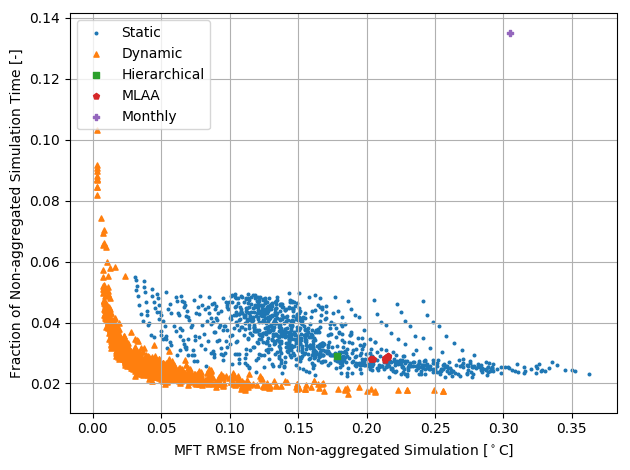
\includegraphics[width=0.95\textwidth]{balanced_1_fraction.png}
\caption{Balanced, 1-year parametric simulation results.}
\label{fig:b1}
\end{figure}

\begin{figure}[htbp!]
\centering
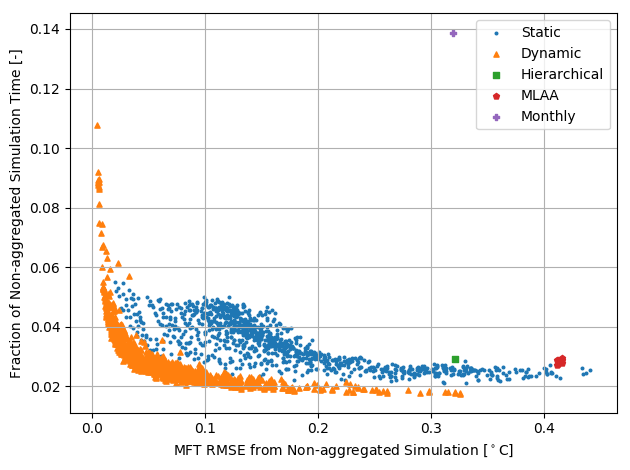
\includegraphics[width=0.95\textwidth]{imbalanced_1_fraction.png}
\caption{Imbalanced, 1-year parametric simulation results.}
\label{fig:i1}
\end{figure}

\begin{figure}[htbp!]
\centering
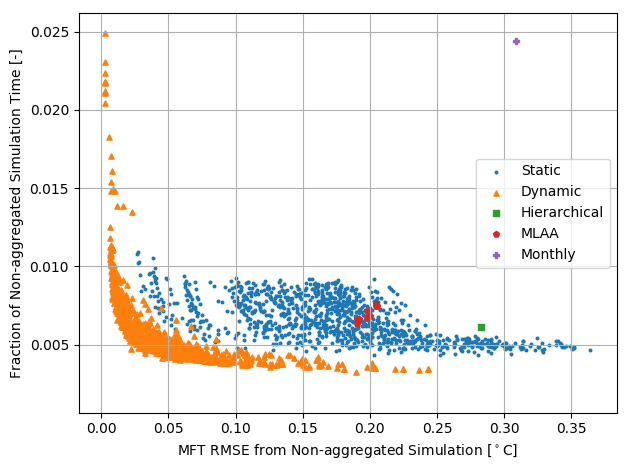
\includegraphics[width=0.95\textwidth]{balanced_5_fraction.png}
\caption{Balanced, 5-year parametric simulation results.}
\label{fig:b5}
\end{figure}

\begin{figure}[htbp!]
\centering
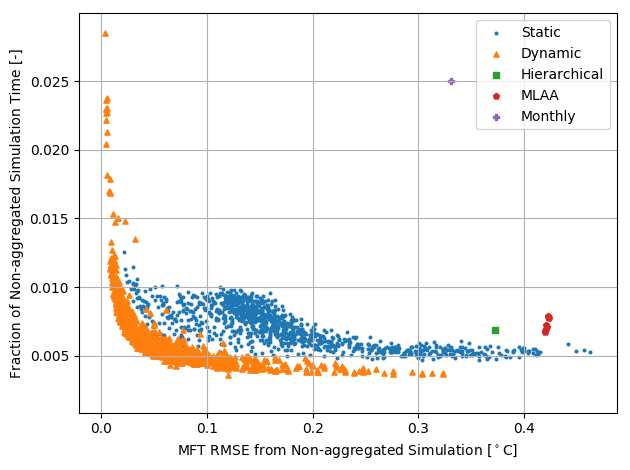
\includegraphics[width=0.95\textwidth]{imbalanced_5_fraction.png}
\caption{Imbalanced, 5-year parametric simulation results.}
\label{fig:i5}
\end{figure}

\section*{Recommendations}

\section*{Conclusions}

\section*{Acknowledgments}
This project was supported under the National Renewable Energy Laboratory Task Order Agreement No.~KAGN-4-42503-00. The computing for the project was performed at the OSU High Performance Computing Center at Oklahoma State University supported in part through the National Science Foundation grant OAC-1126330.

\bibliographystyle{model2-names}\biboptions{authoryear}
\bibliography{references}

\end{document}
